\whiteBGstarBegin
\setcounter{section}{0}
\section{Lý thuyết: Từ trường do dòng điện chạy trong dây dẫn thẳng dài gây ra}
\begin{enumerate}[label=\bfseries Câu \arabic*:]
		\item \mkstar{1} [26]
	
	\cauhoi{
		Viết công thức tính cảm ứng từ tại điểm M trong không khí cách dây dẫn thẳng một đoạn $r$. Cho biết đơn vị các đại lượng có trong công thức. Nếu khoảng cách từ dòng điện đến điểm M tăng lên gấp đôi thì cảm ứng từ tại điểm M thay đổi như thế nào?
		
		
	}
	
	\loigiai{
		
		- Biểu thức tính cảm ứng từ tại điểm M của dòng điện thẳng:  
		
		$$B = 2\cdot 10^{-7} \dfrac{I}{r}$$
		
		- Với 
		
		+ $I$: cường độ dòng điện (A)
		
		+ $B$: Cảm ứng từ (T)
		
		+ $R$: khoảng cách từ điểm M và dòng điện thẳng
		
		- Ta có:
		
		$$B = 2 \cdot 10^{-7} \dfrac{I}{r}.$$
		
		$$B'=2 \cdot 10^{-7} \dfrac{I}{2r}.$$
		
		Suy ra: $$B' =\dfrac{B}{2}.$$
		
	}
	\item \mkstar{2} [23]
	
	\cauhoi{
		Cho dòng điện $\SI{10}{A}$ chạy trong dây dẫn thẳng dài đặt trong không khí. Cảm ứng từ tại điểm M có giá trị bằng $4\cdot 10^{-5}\ \text T$.
		
		\begin{center}
			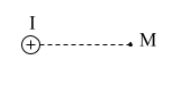
\includegraphics[scale=1]{../figs/VN11-2021-PH-TP021-01.JPG}
		\end{center}
		\begin{enumerate}[label=\alph*)]
			\item Hỏi điểm M cách dây một khoảng là bao nhiêu? 
			\item Biểu diễn vectơ cảm ứng từ tại điểm M.
		\end{enumerate}
		
	}
	
	\loigiai{
		
		\begin{enumerate}[label=\alph*)]
			\item  Khoảng cách từ M đến dây 
			
			$$B = 2 \cdot 10^{-7} \dfrac{I}{r} \Rightarrow r = \SI{0,05}{m}.$$
			
			\item Biểu diễn vectơ cảm ứng từ tại điểm M.
			\begin{center}
				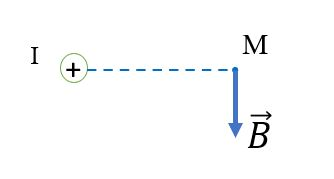
\includegraphics[scale=0.8]{../figs/VN11-2021-PH-TP021-05.JPG}
			\end{center}
			
		\end{enumerate}
	
	}
	
	

	
	\item \mkstar{3} [13]
	
	\cauhoi{
		\begin{minipage}[l]{12cm}
			Hai dây dẫn thẳng song song dài vô hạn đặt cách nhau một khoảng $\SI{14}{cm}$ trong không khí. Dòng điện chạy trong hai dây cùng chiều và có cường độ $I_1 = I_2 = \SI{2,5}{A}$. Đường thẳng CH nằm trong mặt phẳng vuông góc với mặt phẳng chứa hai dây dẫn và là đường trung trực của $I_1I_2$ (như hình vẽ) với  $\text{CH} = \SI{24}{cm}$.  Hãy vẽ vectơ cảm ứng từ tổng hợp tại C và tính độ lớn cảm ứng từ tổng hợp tại C.
		\end{minipage}
		\begin{minipage}[r]{5cm}
			\begin{center}
				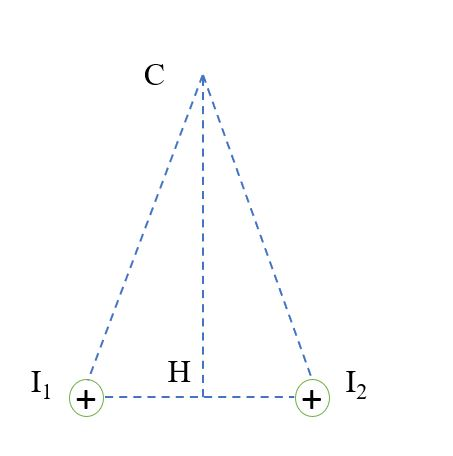
\includegraphics[scale=0.6]{../figs/VN11-2021-PH-TP021-02.JPG}
			\end{center}
		\end{minipage}
		
	}
	
	\loigiai{
		
		\begin{center}
			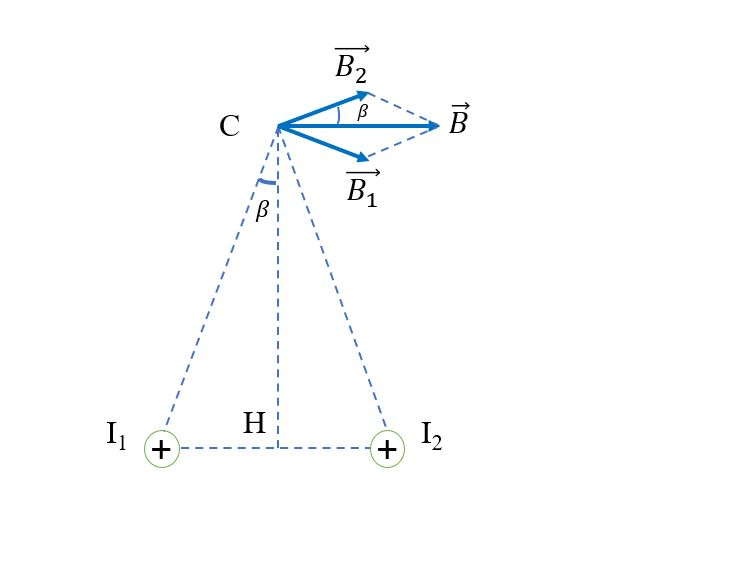
\includegraphics[scale=0.7]{../figs/VN11-2021-PH-TP021-03.JPG}
		\end{center}
		
		Ta có: $$ \vec B = \vec B_1 + \vec B_2.$$
		
		Do C là trung điểm của $I_1I_2$.
		
		Cảm ứng từ của $I_1$ và $I_2$ 
		
		$$B_1=B_2 = 2\cdot 10^{-7} \dfrac{I_1}{r_1} = 2 \cdot 10^{-6}\ \text{T}.$$
		
		Lại có: 
		
		$$\cos \beta = \dfrac{\text{CH}}{I_1\text{C}}.$$
		
		Cảm ứng từ tổng hợp 
		
		$$B=2B_1 \cos \beta= 3,84 \cdot 10^{-6}\ \text T.$$
		
	}
	\item \mkstar{3} [25]
	
	\cauhoi{
		
		Hai dây dẫn thẳng song song dài vô hạn đặt cách nhau $\SI{4}{cm}$ trong không khí. Dòng điện chạy trong hai dây là $I_1=\SI{10}{A}$; $I_2=\SI{20}{A}$ và ngược chiều nhau. Xác định hướng và độ lớn cảm ứng từ tại điểm M cách mỗi dây là $\SI{2}{cm}$.
		
		
	}
	\loigiai{
		
		\begin{center}
			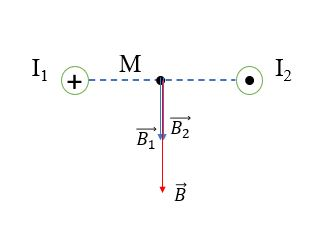
\includegraphics[scale=0.9]{../figs/VN11-2021-PH-TP021-04.JPG}
		\end{center}
		
		Cảm ứng từ của $I_1$ tác dụng lên M
		
		$$B_1 = 2 \cdot 10^{-7} \dfrac{I_1}{r_1} = 10^{-4}\ \text{T}.$$
		
		Cảm ứng từ của $I_2$ tác dụng lên M
		
		$$B_1 = 2 \cdot 10^{-7} \dfrac{I_1}{r_1} = 2 \cdot 10^{-4}\ \text{T}.$$
		
		Cảm ứng từ tổng hợp tại M
		
		$$ \vec B = \vec B_1 + \vec B_2$$
		
		Do $\vec B_1$ cùng hướng với $\vec B_2$ nên suy ra
		
		$$B = B_1+B_2 =3 \cdot 10^{-4}\ \text T.$$
		}
	
\end{enumerate}
\section{Lý thuyết: Từ trường do dòng điện chạy trong khung dây dẫn tròn hoặc trong ống dây hình trụ gây ra}
\begin{enumerate}[label=\bfseries Câu \arabic*:]
	
	\item \mkstar{2}
	
	\cauhoi{
		
		Khi cho dòng điện cường độ $\SI{10}{A}$ chạy qua một vòng dây dẫn đặt trong không khí thì cảm ứng từ tại tâm của vòng dây dẫn có độ lớn là $\text{2,1}\cdot 10^{-4}\ \text{T}$. Xác định bán kính của vòng dây.
		\begin{mcq}(4)
			\item $\SI{5,0}{cm}.$
			\item $\SI{0,3}{cm}.$
			\item $\SI{3,0}{cm}.$
			\item $\SI{2,5}{cm}.$
		\end{mcq}
	}
	\loigiai{
		
		\textbf{Đáp án: C.}
		
		Bán kính vòng dây  
		
		$$B = 2 \pi \cdot 10^{-7} \dfrac{I}{R} \Rightarrow R =  2 \pi \cdot 10^{-7} \dfrac{I}{B} = \SI{0,03}{m}.$$
	}	
	
	
	
		\item \mkstar{2}
		\cauhoi{
			
			Một vòng dây tròn đặt trong chân không có bán kính $R$ mang dòng điện có cường độ $I$ thì cảm ứng từ tại tâm vòng dây là $10\ \mu \text{T}$. Nếu cho dòng điện trên qua vòng dây có bán kính $4R$ thì cảm ứng từ tại tâm vòng dây có độ lớn là
			\begin{mcq}(4)
				\item $6 \cdot 10^{-6}\ \text{T}$.
				\item $\text{1,2}\cdot 10^{-6}\ \text{T}.$	
				\item $15 \cdot 10^{-6}\ \text{T}$.		
				\item $\text{2,5}\cdot 10^{-6}\ \text{T}.$	
			\end{mcq}
		}
		\loigiai{
			
			\textbf{Đáp án: D.}
			
			Ta có: 
			
			$$\dfrac{B_1}{B_2}= \dfrac{4R}{R} \Rightarrow B_2 = \dfrac{B_1}{4} =\text{2,5}\cdot 10^{-6}\ \text T. $$
		}	
	
		\item \mkstar{3}
		\cauhoi{
			
			Dùng một dây đồng có phủ một lớp sơn cách điện mỏng, quấn quanh một hình trụ dài $L = 50\ \text{cm}$, có đường kính $d = 4\ \text{cm}$ để làm một ống dây. Sợi dây quấn ống dây có chiều dài $l = 314\ \text{cm}$ và các vòng dây được quấn sát nhau. Hỏi nếu cho dòng điện cường độ $I = \text{0,4}\ \text{A}$ chạy qua ống dây, thì cảm ứng từ bên trong ống dây bằng bao nhiêu?
			\begin{mcq}(4)
				\item $5 \cdot 10^{-5}\ \text{T}$.			
				\item $\text{2,5}\cdot 10^{-5}\ \text{T}.$		
				\item $\text{1,25}\cdot 10^{-5}\ \text{T}.$		
				\item $3 \cdot 10^{-5}\ \text{T}$.	
			\end{mcq}
		}
		\loigiai{
			
			\textbf{Đáp án: B.}
			
			Chu vi của mỗi vòng dây $\pi d$.
			
			Số vòng dây
			
			$$N = \dfrac{l}{\pi d}.$$
			
			Cảm ứng từ tại bên trong ống dây
			
			$$B = 4 \pi \cdot 10^{-7} \dfrac{NI}{L}= 4  \cdot 10^{-7} \dfrac{ lI}{Ld} = \text{2,5} \cdot 10^{-5}\ \text{T}.$$
		}	

	
		\item \mkstar{1} [19]
	
	\cauhoi{
		
		Nêu công thức tính cảm ứng từ tại tâm của một khung dây dẫn tròn đặt trong không khí (có chú thích các đại lượng trong công thức).
		
	}
	
	\loigiai{
		
		+ Biểu thức: $$B = 2\pi \cdot 10^{-7} N \dfrac{I}{R}$$
		
		$N$: số vòng dây của khung.
		
		$I$: cường độ dòng điện qua khung.
		
		$R$: bán kính khung dây.
		
	}
\end{enumerate}

\whiteBGstarEnd